%!TEX root = thesis.tex

\chapter{Introduction}

The advent of multi-core architectures has emphasized the crucial importance of mechanisms supporting correct and scalable multi-threaded programming.
In this model, threads can collaborate by interacting on data structures (such as tables, message queues, buffers, etc.) maintained in shared memory.

Traditional lock-based mechanisms (like mutex constructs, semaphores, and barriers) used to regulate access to these shared data are notoriously difficult and error-prone, as they easily lead to deadlocks, race conditions and priority inversions; moreover, they are not composable and hinder parallelism, thus reducing efficiency and scalability.
\emph{Transactional memory} (TM) has emerged as a promising mechanism to replace locks \cite{moss:transactionalmemorybook,st:dc1997}.  The basic idea is to mark blocks of code as \emph{atomic}; then, execution of each block will appear either if it was executed instantaneously at some unique point in time, or, if aborted, as if it did not execute at all. This is obtained by means of \emph{optimistic} executions: the blocks are allowed to run concurrently, and eventually if an interference is detected a transaction is restarted and its effects are rolled back.
Transactions are composable and ensure absence of deadlocks and  priority inversions, automatic roll-back on exceptions, and increased concurrency.  Each transaction can be viewed in isolation as a \emph{single-threaded} computation, significantly reducing programmer's burden.

\section{Motivations}

In multi-threaded programming different transactions may need to interact and exchange data \emph{before} committing.
In this situation, transaction isolation is a severe shortcoming.
A simple example is a request-response interaction via a shared buffer.
We could try to synchronize the threads accessing the buffer \emph{b} by means of two semaphores \verb|c1|, \verb|c2| as follows:
\begin{figure}[h]
\centering
\begin{minipage}[t]{0.4\textwidth}
\begin{BVerbatim}[baseline=t]
// Party1 (Master)
atomically {
  // put request in b
  up(c1);
  // some other code
  down(c2);
  // get answer from b
}
\end{BVerbatim}
\end{minipage}
\begin{minipage}[t]{0.3\textwidth}
\begin{BVerbatim}[baseline=t]
// Party2 (Worker)
atomically {
  // some code before
  down(c1);
  // get request from b
  // put answer in b
  up(c2);
  // some code after
}
\end{BVerbatim}
\end{minipage}
\end{figure}
\newpage
Unfortunately, this solution does not work: any admissible execution requires an interleaved scheduling between the two transactions, thus violating isolation; hence, the transactions deadlock as none of them can progress.
It is important to notice that this deadlock arises because synchronization occurs between threads in \emph{different} transactions;
in fact, the solution above is perfectly fine for threads \emph{outside} transactions, or within the \emph{same} transaction.

\section{Thesis proposal}
In order to overcome this limitation, in this thesis we propose a programming model for \emph{safe, data-driven} interactions between memory transactions.
The key observation is that \emph{atomicity} and \emph{isolation} should be seen as two disjoint computational aspects:
\begin{itemize}
\item an atomic \emph{non-isolated} block of code is executed ``all-or-nothing'', but its execution can overlap that of others and \emph{uncontrolled} access to shared data is allowed;
\item an \emph{isolated} block of code is intended to be executed ``as it were the only one'' (i.e., in mutual exclusion with other threads), but no rollback on errors/exceptions is provided.
\end{itemize}
Thus, a ``normal'' block of code is neither atomic nor isolated; a mutex block (like Java \emph{synchronized} methods) is isolated but not atomic; and a usual transaction is a block which is both atomic and isolated.
Atomic non-isolated blocks can be used for implementing safe composable interacting memory transactions, henceforth called \emph{open transactions}.

In this model, a transaction is composed by several threads, called \emph{participants}, which can cooperate on shared data.  A transaction commits when all its participants commit, and aborts if any thread aborts.  Threads participating to different transactions can access to shared data, but when this happens the transactions are \emph{transparently merged} into a single one.  For instance, the two transactions of the synchronization example above would automatically merge becoming the same transaction, so that the two threads can synchronize and proceed.  Thus, this model relaxes the isolation requirement still guaranteeing atomicity and consistency; moreover, it allows for \emph{loosely-coupled} interactions since transaction merging is driven only by run-time accesses to shared data, without any explicit coordination among the participants beforehand.

These concepts have already been presented in \cite{MiculanPT15,Toneguzzo,OpenTransactionsSpec}, so in this thesis we will not present the operational semantics of the model and the \emph{opacity} correctness criterion\cite{gk:ppopp08}.

In summary, the contributions of this thesis are the following:
\begin{itemize}
\item We present \emph{Open Transactional Memory}, a transactional memory model where multi-threaded transactions can interact by non-isolated access to shared data. Consistency and atomicity are ensured by transparently \emph{merging} transactions at runtime.

\item We describe this model in the context of Concurrent Haskell (\cref{chap:otm}).
We define two monads \emph{OTM} and \emph{ITM}, representing the computational aspects of atomic \emph{multi-threaded open} (i.e., non-isolated) transactions and atomic \emph{single-threaded isolated} transactions, respectively (Figure~\ref{fig:acid-spectrum}).
Using the construct \emph{atomic}, programs in the \emph{OTM} monad are executed ``all-or-nothing'' but without isolation; hence these transactions can merge at runtime.
When needed, isolation inside transactions can be guaranteed by the construct \textcode{isolated}.
Both OTM and ITM transactions are \emph{composable},
and we exploit Haskell type system to forbid irreversible effects inside these two monads.

\item We illustrate the effectiveness of this programming model by providing several example implementations, such as barriers, \emph{futures} and Petri nets, among others.
Moreover, \emph{OTM} is a conservative extension 
of \emph{STM} \citep{Harris:2005:CMT:1065944.1065952}; in fact, \emph{atomically} is precisely the composition of \emph{atomic} and \emph{isolated} (Figure~\ref{fig:acid-spectrum}).

\item We give an implementation of OTM as a library for Concurrent Haskell (\cref{chap:implementation}).  Ours is a pure software implementation using some functionalities of the Haskell Runtime System, and does not require any change in the compiler or the runtime environment. Furthermore, our implementation can be easily integrated in the Runtime System with minimal changes to STM data structures.
\end{itemize}


\begin{figure}
    \centering
    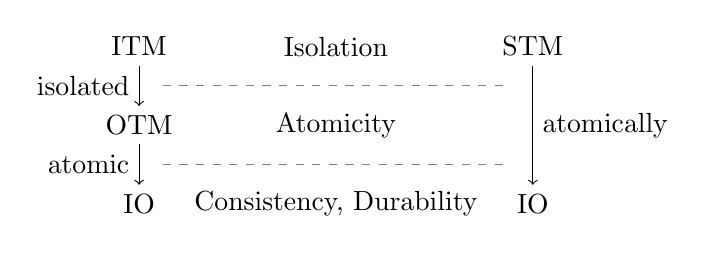
\begin{tikzpicture}
        \node[] (n00) at (0,0) {IO};
        \node[] (n01) at (0,1) {OTM};
        \node[] (n02) at (0,2) {ITM};

        \draw[->] (n02) to node[left] {\textcode{isolated}} (n01);
        \draw[->] (n01) to node[left] {\textcode{atomic}} (n00);

        \node[] (n20) at (5,0)  {IO};
        \node[] (n21) at (5,2){STM};

        \draw[->] (n21) to node[right] {\textcode{atomically}} (n20);

        \node[] (n10) at (2.5,0) {Consistency, Durability};
        \node[] (n11) at (2.5,1) {Atomicity};
        \node[] (n12) at (2.5,2) {Isolation};

        \draw[gray,dashed] (.3,.5) -- (4.7,.5);
        \draw[gray,dashed] (.3,1.5) -- (4.7,1.5);
    \end{tikzpicture}
    \caption{ACID computations: splitting \textcode{atomically}.}
    \label{fig:acid-spectrum}
\end{figure}

\section{Synopsis}
\begin{itemize}
\item In the \cref{chap:haskell} we illustrate the Haskell programming language and the solutions it provides for internal concurrency.

\item In the \cref{chap:otm} we present the programming interface of the OTM model among several example implementations of synchronization primitives and coordination paradigms.

\item In the \cref{chap:ghc} we give an overview of the Haskell compiler, the runtime support and the STM implementation.

\item In the \cref{chap:implementation} we illustrate the implementation of the OTM model.

\item Conclusions and possible future works are illustrated in \cref{chap:conc}.
\end{itemize}
